\scanpage{43}
$T_r\quad(=T^{(p^r)})$
\margin{\figure{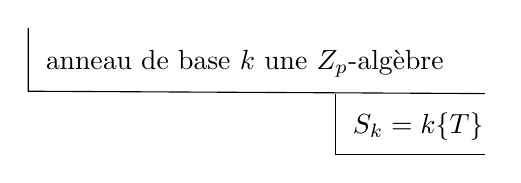
\begin{tikzpicture}[x=1cm,y=1cm]\node[anchor=west] at (.1,.35) {anneau de base $k$ une $\mathbb Z_p$-algèbre};\draw (0,.8)--(0,0)--(5.8,-.03);\node[anchor=west] at (4,-.45) {$S_k=k\{T\}$};\draw (3.9,-.03)--(3.9,-.8)--(5.8,-.8);\end{tikzpicture}}}
\[
T_r^p=p!(T^{(p^r)})^{(p)}=p!\underset{\substack{\Vert\\\frac{p^{r+1}!}{(p^r!)^p p!}\in\mathbb Z_p^*}}{\nu_r}T^{(p^{r+1})}=p\nu'_rT_{r+1}
\]
\[
\nu'_r=(p-1)!\frac{p^{r+1}!}{(p^r!)^p p!}\in\mathbb Z_p^*
\]
\[
\boxed{T_r^p=p\underset{\substack{\cap\\\mathbb Z_p^*}}{\nu'_r}T_{r+1}}
\]
$\tau_{p^r}S_k$ a comme base les $T_{\unsure{\bullet|*}}^{\uline{i}}$, $\uline{i}=(i_0,i_1,\cdots,i_r,i_{r+1},\cdots$
\[
\text{où}\quad\sum i_\alpha p^\alpha\geq p^r\quad\text{i.e.}\quad\exists\alpha\geq r\ \text{avec}\ i_\alpha\ne0
\]
Donc $\tau_{p^r}S$ est engendré par $\underset{\substack{\Vert\\t_r}}{T_r},\underset{\substack{\Vert\\t_{r+1}}}{T_{r+1}},\cdots,\underset{\ell\geq0}{T_{r+\ell}},\cdots$

les relations sont
\[
\boxed{T_s^{p-1}t_s=p\nu'_s t_{s+1}\qquad\text{si }s\geq r}.
\]
donc un hom de degré $d<p^r$, $d=d_0+d_1p\cdots+d_{r-1}p^{r-1}$
\diagram{\begin{tikzcd}
u:\tau_{p^r}S_k\arrow[r] & \unsure{M|N}\otimes_k S_k
\end{tikzcd}}
est donné par \unsure{des}
\[
\deleted{(\unsure{R_s})}\qquad\boxed{u(t_s)=\deleted{\unsure{\xi_s}T^{(p^s-d)}}\eta_s\in S_{\unsure{k}}^{(p^s-d)}\otimes_k M}
\]
avec les relations
\[
(R_s)\qquad\boxed{T_s^{p-1}\eta_s=p\nu'_s\eta_{s+1}}
\]
Soit $\nu=\unsure{\nu_p|v_p}(d)$ de sorte que
\[
d=d_\nu p^\nu\cdots+d_{r-1}p^{r-1}=p^\nu(d_\nu+d_{\nu+1}p\cdots+d_{r-1}p^{r-1-\nu}
\]
$d_\nu\ne0$ i.e. $d_\nu\geq1$
\[
p^s-d=p^\nu\left(p^{s-\nu}-\frac d{p^\nu}\right)=p^\nu\left(p^{s-\nu}-1-\underbrace{\left(\frac d{p^\nu}-1\right)}_{(d_\nu-1)+d_{\nu+1}p\cdots+d_{r-1}p^{r-1-\nu}}\right.
\]
\[
=p^\nu\left(\underset{\substack{\Vert\\(p-1)-(d_\nu-1)}}{\delta_\nu}+\underset{\substack{\Vert\\(p-1)-d_{\nu+1}}}{\delta_{\nu+1}}p\cdots+\underset{\substack{\Vert\\(p-1)-(d_{r-1})}}{\delta_{r-1}}p^{r-\nu-1}+\underbrace{(p-1)p^{r-\nu}+(p-1)p^{r-\nu+1}+\cdots+(p-1)p^{s-\nu-1}}_{\text{si }s>r}\right.
\]
donc $S^{(p^s-d)}$ a comme base
\[
\deleted{\unsure{T_\beta}}T_\nu^{\delta_\nu}T_{\nu+1}^{\delta_{\nu+1}}\cdots T_{r-1}^{\delta_{r-1}}(T_r^{\deleted{\unsure{p-1}}}\cdots T_{s-1})^{p-1}
\]
\margin{$\longrightarrow$ à facteur \unsure{inv. près} si $s>r$}
\mspage{42}
